%
% .tex file needs 6_17.jpg, 6_19.jpg, and F6_26.jpg
%

\documentclass[12pt,letterpaper,boxed]{hmcpset}
\usepackage[margin=1 in]{geometry}
\usepackage{graphicx}
\usepackage{courier}
\usepackage{tabto}
\usepackage{amsmath, amssymb}
\usepackage{subfig}
\usepackage{framed}
\usepackage{enumerate}
\usepackage{pdfsync}
\usepackage{mathtools}
\usepackage{caption}
\usepackage{booktabs}
\usepackage{listings}
\usepackage{siunitx, xfrac}
\usepackage{color}



\definecolor{mygreen}{rgb}{0,0.6,0}
\definecolor{mygray}{rgb}{0.5,0.5,0.5}
\definecolor{mymauve}{rgb}{0.58,0,0.82}

\lstset{ %
  backgroundcolor=\color{white},     % choose the background color; you must add \usepackage{color} or \usepackage{xcolor}
  basicstyle=\footnotesize\ttfamily, % the size of the fonts that are used for the code
  breakatwhitespace=false,           % sets if automatic breaks should only happen at whitespace
  breaklines=true,                   % sets automatic line breaking
  captionpos=b,                      % sets the caption-position to bottom
  commentstyle=\color{mygreen},      % comment style
  deletekeywords={...},              % if you want to delete keywords from the given language
  escapeinside={\%*}{*)},            % if you want to add LaTeX within your code
  extendedchars=true,                % lets you use non-ASCII characters; for 8-bits encodings only, does not work with UTF-8
  frame=single,                      % adds a frame around the code
  keepspaces=true,                   % keeps spaces in text, useful for keeping indentation of code (possibly needs columns=flexible)
  keywordstyle=\color{blue},         % keyword style
  language=Octave,                   % the language of the code
  morekeywords={*,...},              % if you want to add more keywords to the set
  numbers=left,                      % where to put the line-numbers; possible values are (none, left, right)
  numbersep=5pt,                     % how far the line-numbers are from the code
  numberstyle=\tiny\color{mygray},   % the style that is used for the line-numbers
  rulecolor=\color{black},           % if not set, the frame-color may be changed on line-breaks within not-black text (e.g. comments (green here))
  showspaces=false,                  % show spaces everywhere adding particular underscores; it overrides 'showstringspaces'
  showstringspaces=false,            % underline spaces within strings only
  showtabs=false,                    % show tabs within strings adding particular underscores
  stepnumber=2,                      % the step between two line-numbers. If it's 1, each line will be numbered
  stringstyle=\color{mymauve},       % string literal style
  tabsize=2,                         % sets default tabsize to 2 spaces
}

\name{Jerry Hsiung}
\class{Computer Vision 16-720}
\assignment{Assignment 4}
\duedate{\today}

\begin{document}
\problemlist{Assignment \#4}

%%%%%%%%%%%%%%%%%%%%%%%%%%%%%%%%%
%		1
%%%%%%%%%%%%%%%%%%%%%%%%%%%%%%%%%
\begin{problem}[]
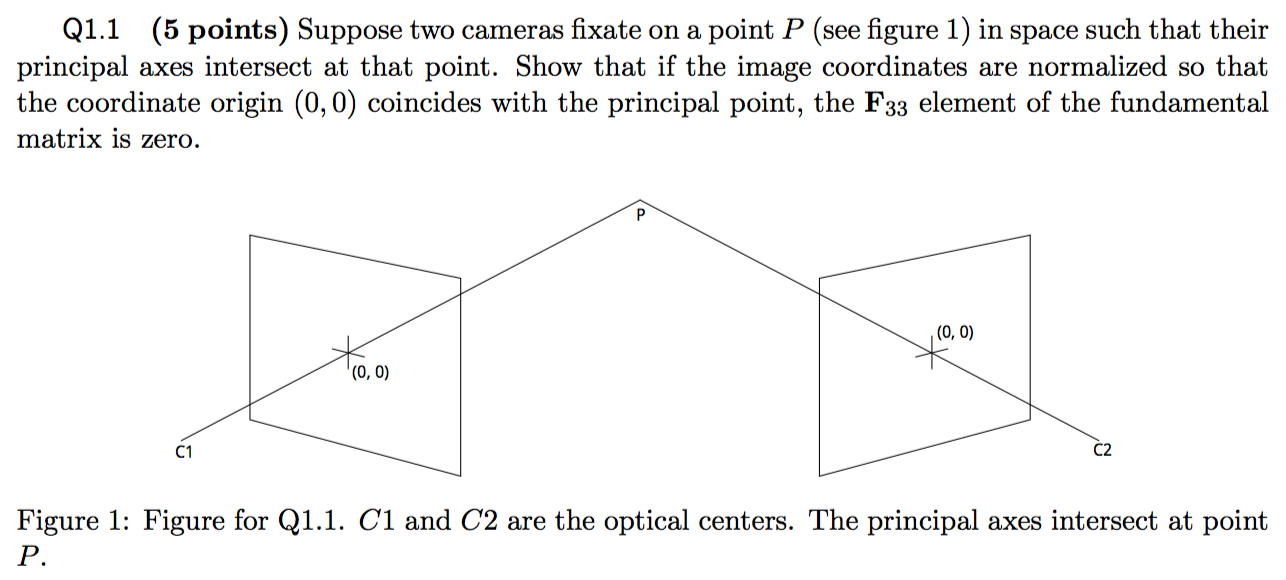
\includegraphics[width=\textwidth]{1_1.png}
\end{problem}

\begin{solution}
Let $\mathbf{x'} = [x', y', 1]^T, \mathbf{x} = [x, y, 1]^T$. According to the definition of fundamental matrix:
\begin{align*}
  \mathbf{x}'F\mathbf{x} &= 0\\
  x'xf_{11} + x'yf_{12} + x'f_{13} +
  y'xf_{21} + y'yf_{22} + y'f_{23} +
  xf_{31} + yf_{32} + f_{33}  &= 0
\end{align*}
Given that the coordinate are normalized, and $x' = x = (0,0)$, then to make the equation hold true is when $f_{33} = 0$.
\end{solution}

\begin{problem}[]
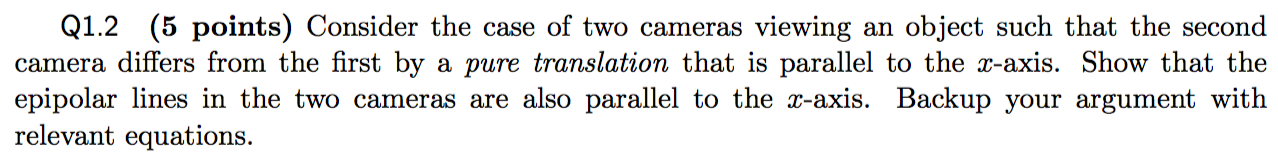
\includegraphics[width=\textwidth]{1_2.png}
\end{problem}
\begin{solution}
Suppose the camera frame 1 is the origin, the camera frame 2 has rotation $R = I$ and translation $t$ with respect to frame 1. The point $\mathbf{x}_2$ in frame 2 can be written as $R\mathbf{x}_1+t = \mathbf{x}_1+t$. Also, since camera 1 is at the origin, then frame 2's epipole $\mathbf{e}_2 = t$. Now, denoted the epipolar lines in two camera frames $l_1, l_2$, then using the definition of epipolar line,
we get $l_2 = [\mathbf{e}_2]_\times \mathbf{x}_2$. We can rewrite this definition and get:
\begin{align*}
  l_2 &= [\mathbf{e}_2]_\times \mathbf{x}_2\\
      &= [t]_\times (R\mathbf{x}_1+t)\\
      &= [t]_\times\mathbf{x}_1 + [t]_\times t &\text{(Since $R = I$)}\\
      &= [t]_\times\mathbf{x}_1 &\text{(Cross product of itself $ = 0$)}\\
\end{align*}
Supposed there is a point $t$ in frame 2, using triple scalar product:
\begin{align*}
  l_2 &= [t]_\times\mathbf{x}_1 &\text{(Cross product of itself $ = 0$)}\\
  t \cdot l_2 &= t \cdot [t]_\times\mathbf{x}_1 \\
              &= 0
\end{align*}
This means that the point $t$ and the line $l_2$ is, in fact, colinear. And since point $t$ can
be treated as vector $t$ from the origin in frame 2, the results tells us that the vector $t$ is
colinear, and therefore, parallel to $l_2$. This shows that the epipolar line $l_2$ is parallel to the translation $t$, in this case x-axis. 

Similar to analyze $l_1$, we can treated frame 2 as the origin, then the translation $t$ is just the negative
direction of x-axis. Then follow the similar analysis, we can see that $l_1 = [-t]_\times\mathbf{x}_1$, and is also
parallel to the x-axis.
\end{solution}

\begin{problem}[]
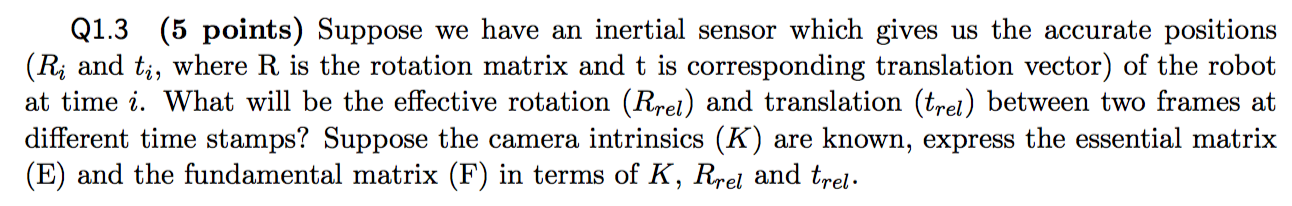
\includegraphics[width=\textwidth]{1_3.png}
\end{problem}
\begin{solution}
The relative rotation will be: $R_{rel} = \frac{R_{i+1}}{R_i}$\\
and translatoin will be: $t_{rel} = t_{i+1}-{t_i}$.\\

Since the first camera is now the original frame, the camera matrices $P, P'$ are $K[\mathbf{I}|0], K[\mathbf{R}|t]$. Given the definition of fundamental matrix from the text book, we can write $F$ as:
\begin{align*}
  F &= K^{-T}[\mathbf{t_{rel}}]_\times R_{rel}K^{-1}\\
  E &= K^{T}FK\\
    &= K^{T}[K^{-T}[\mathbf{t_{rel}}]_\times R_{rel}K^{-1}]K\\
    &= [\mathbf{t_{rel}}]_\times R_{rel}
\end{align*}
\end{solution}

\begin{problem}[]
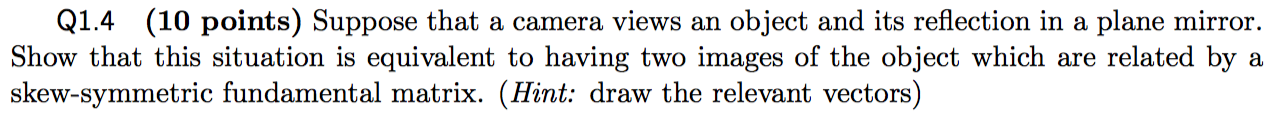
\includegraphics[width=\textwidth]{1_4.png}
\end{problem}
\begin{solution}
Looking at below picture, \\
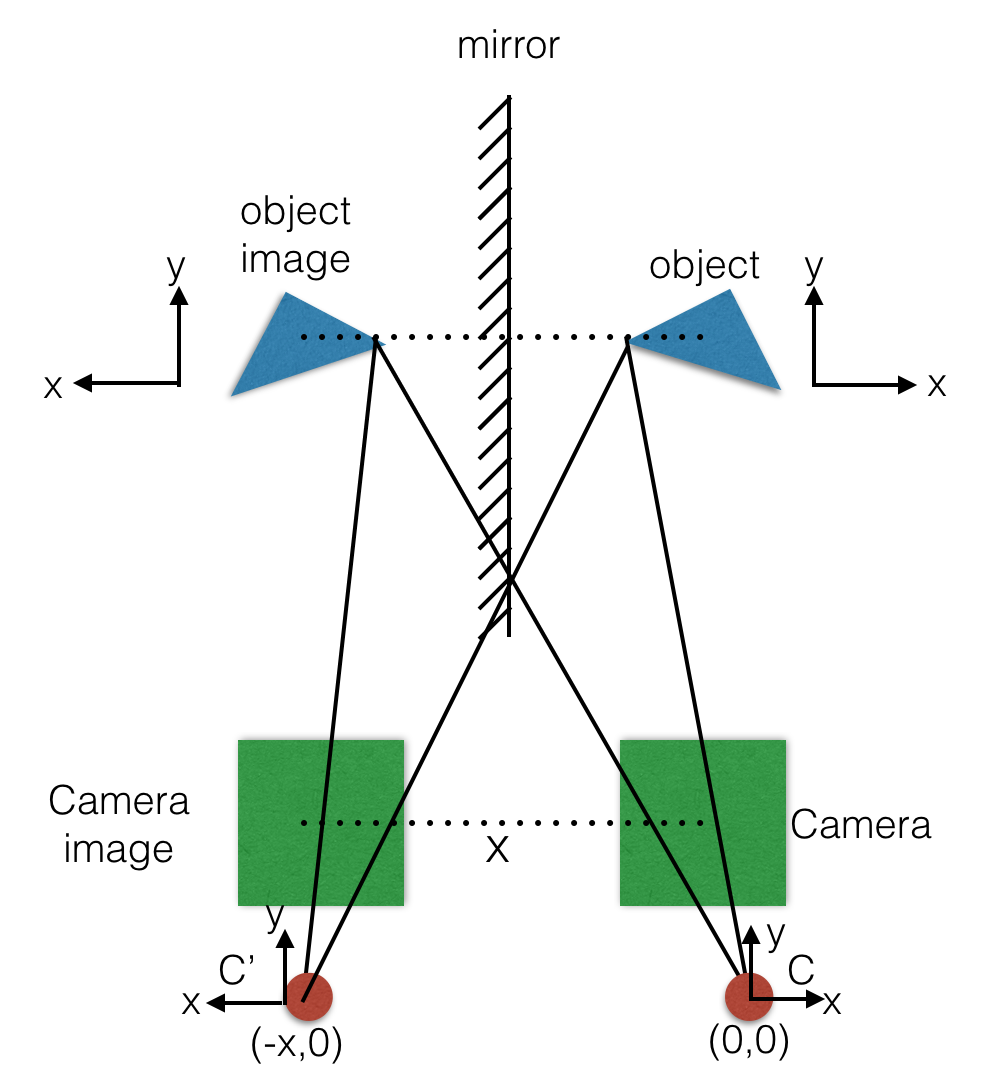
\includegraphics[width=0.5\textwidth]{1-4.png}\\
the problem can be seen that the object has flip the axis
before and after the reflection of the mirror. Since the vector of the object and its mirror image
is always perpendicular to the mirror (parallel to the normal of the mirror), then 
we can always define the coordinate system such that the x-axis is flip of the object and its 
mirror image. 

Looking at an object that the x-axis is flip, we can instead flip the camera object into the mirror on the x-axis with some 
translation $t= [x, 0, 0]^T$ since we define the axis perpendicular to the mirror is $x$.
Therefore, assuming the original camera is at $[I|0]$, and the second to be $[R|t]$, so its original rotation:
\[
 I = R = \begin{pmatrix}
   1 & 0 & 0\cr
   0 & 1 & 0\cr
   0 & 0 & 1\cr
  \end{pmatrix} \\
\]
 , then the second camera rotation can be seen as
 \[
 R' = \begin{pmatrix}
   -1 & 0 & 0\cr
   0 & 1 & 0\cr
   0 & 0 & 1\cr
  \end{pmatrix} \\
\]
The definition of the fundamental matrix is 
\begin{align*}
  F &=  K'^{-1} [t]_\times RK^{-1} &\text{($K' = K$, since it is the same camera)}\\
    &= 
   K'^{-T}  [t]_\times
  \begin{pmatrix}
   -1 & 0 & 0\cr
   0 & 1 & 0\cr
   0 & 0 & 1\cr
  \end{pmatrix} K^{-1}\\
\end{align*}
Using the definition of skew symmetric, we have:
\begin{align*}
  -F &= K'^{-T}  -[t]_\times
  \begin{pmatrix}
   -1 & 0 & 0\cr
   0 & 1 & 0\cr
   0 & 0 & 1\cr
  \end{pmatrix} K^{-1}\\
     &= 
  K'^{-T}  ([t]_\times)^T
  \begin{pmatrix}
   -1 & 0 & 0\cr
   0 & 1 & 0\cr
   0 & 0 & 1\cr
  \end{pmatrix} K^{-1} &\text{(since $[t]_\times$ is skew-symmetric)}\\
     &= 
  K'^{-T}  ([t]_\times)^T
  (\begin{pmatrix}
   -1 & 0 & 0\cr
   0 & 1 & 0\cr
   0 & 0 & 1\cr
  \end{pmatrix})^T K^{-1}\\
    &= 
  K'^{-T}(
  \begin{pmatrix}
   -1 & 0 & 0\cr
   0 & 1 & 0\cr
   0 & 0 & 1\cr
  \end{pmatrix}[t]_\times)^T K^{-1}\\
   &= 
  (K'^{-T}
  \begin{pmatrix}
   -1 & 0 & 0\cr
   0 & 1 & 0\cr
   0 & 0 & 1\cr
  \end{pmatrix}[t]_\times K^{-1})^T\\
     &= 
  (K'^{-T}[t]_\times
  \begin{pmatrix}
   -1 & 0 & 0\cr
   0 & 1 & 0\cr
   0 & 0 & 1\cr
  \end{pmatrix} K^{-1})^T &\text{(since $t$ only has $x$ component)}\\
  &= F^T
\end{align*}
And therefore we have shown that $F$ is skew-symmetric.
\end{solution}

\begin{problem}[2.1]
Write down recovered $F$, and a screen shot of the eight-point algorithm
\end{problem}
\begin{solution}
My recovered $F$ is:
\begin{verbatim} 
F=
  -0.000000387339232  -0.000016376057910   0.230251620507768
  -0.000022365870885   0.000000270614880   0.000712358533553
  -0.221134562248653   0.003244227691014  -0.949034123261248
\end{verbatim}
The example output is also shown below:\\
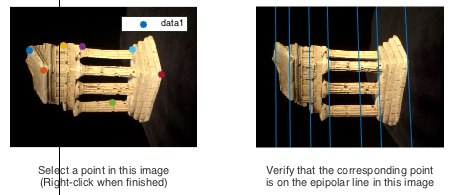
\includegraphics[width=\textwidth]{q2_1.png}
\end{solution}

\begin{problem}[2.2]
Write down recovered $F$, and a screen shot of the seven-point algorithm
\end{problem}
\begin{solution}
The corrected recovered $F$ is:
\begin{verbatim} 
F=
   0.000002359180802  -0.000024943546940   0.119260923224233
   0.000003283957910   0.000000763477904  -0.004834507315101
  -0.115202554620373   0.008647145570517  -0.986203369964319
\end{verbatim}
The example output is also shown below:\\
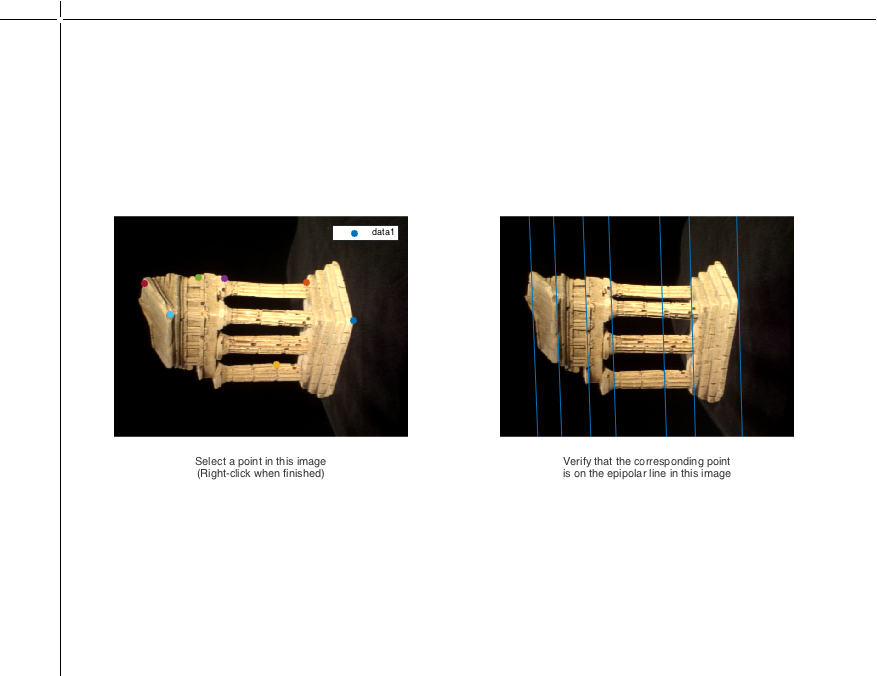
\includegraphics[width=\textwidth]{q2_2.png}
\end{solution}

\begin{problem}[2.3]
Write down the estimated $E$ using the $F$ from the eight-point algorithm
\end{problem}
\begin{solution}
My estimated $E$ is:

\begin{verbatim}
E=
  1.0e+02 *
  -0.008953796271707  -0.379920999744570   3.437499160013362
  -0.518883364564895   0.006300917861968  -0.091286736435895
  -3.447858595398019  -0.025021333457005  -0.001263668309641
\end{verbatim}
\end{solution}

\begin{problem}[2.6]
Include a screenshot of epipolarMatchGUI with some detected correspondances
\end{problem}
\begin{solution}
Below is the graph showing the correspondances. Note that ALL of the points are 
estimated correctly, but most of them are close enough for 3D reconstruction for
the next section:\\
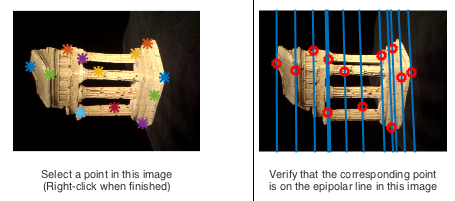
\includegraphics[width=\textwidth]{q2_6.png}
\end{solution}


\begin{problem}[2.7]
Screenshots of the 3D visualization of the temple.
\end{problem}
\begin{solution}
Since my triangulation method is not optimizing the 3D reprojection,
the results for my 3D reconstruction is not perfect. However, the overall
shape of the temple and its 3D positions are clearly visible in the below graphs:\\
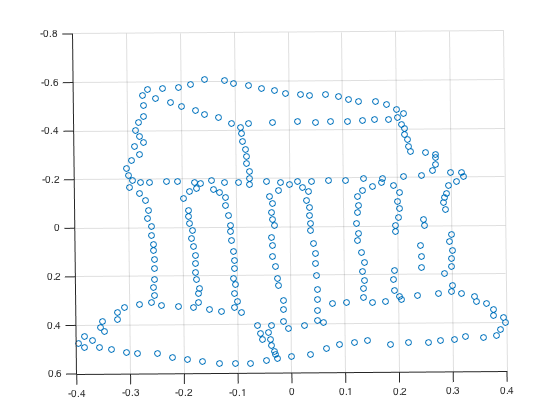
\includegraphics[width=0.5\textwidth]{q2_7_1.png}
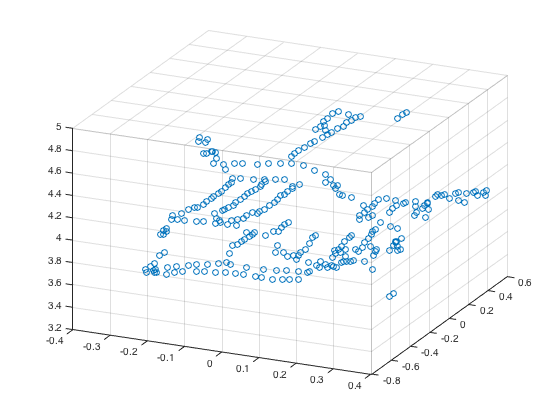
\includegraphics[width=0.5\textwidth]{q2_7_2.png}\\
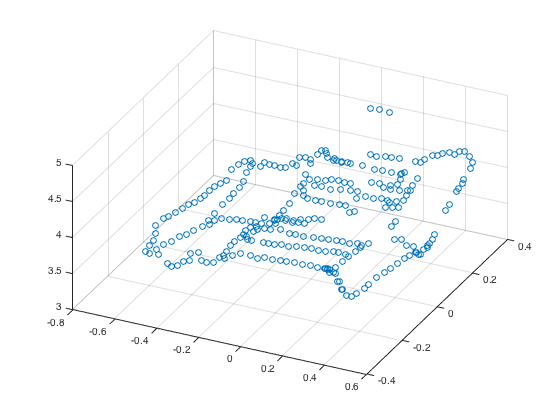
\includegraphics[width=0.5\textwidth]{q2_7_3.png}
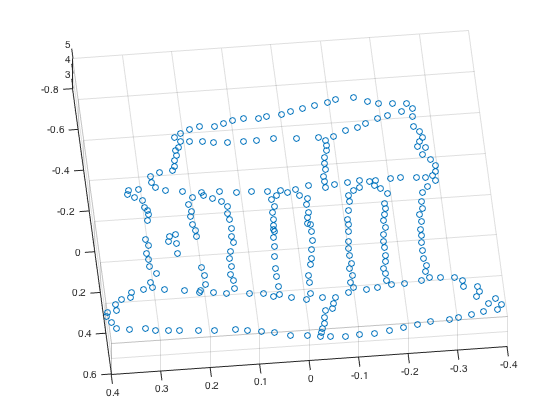
\includegraphics[width=0.5\textwidth]{q2_7_4.png}

\end{solution}


\end{document}


